\section{Concept Design}
\label{sec:Concept_Design}

\begin{figure}[!htb]
\begin{center}
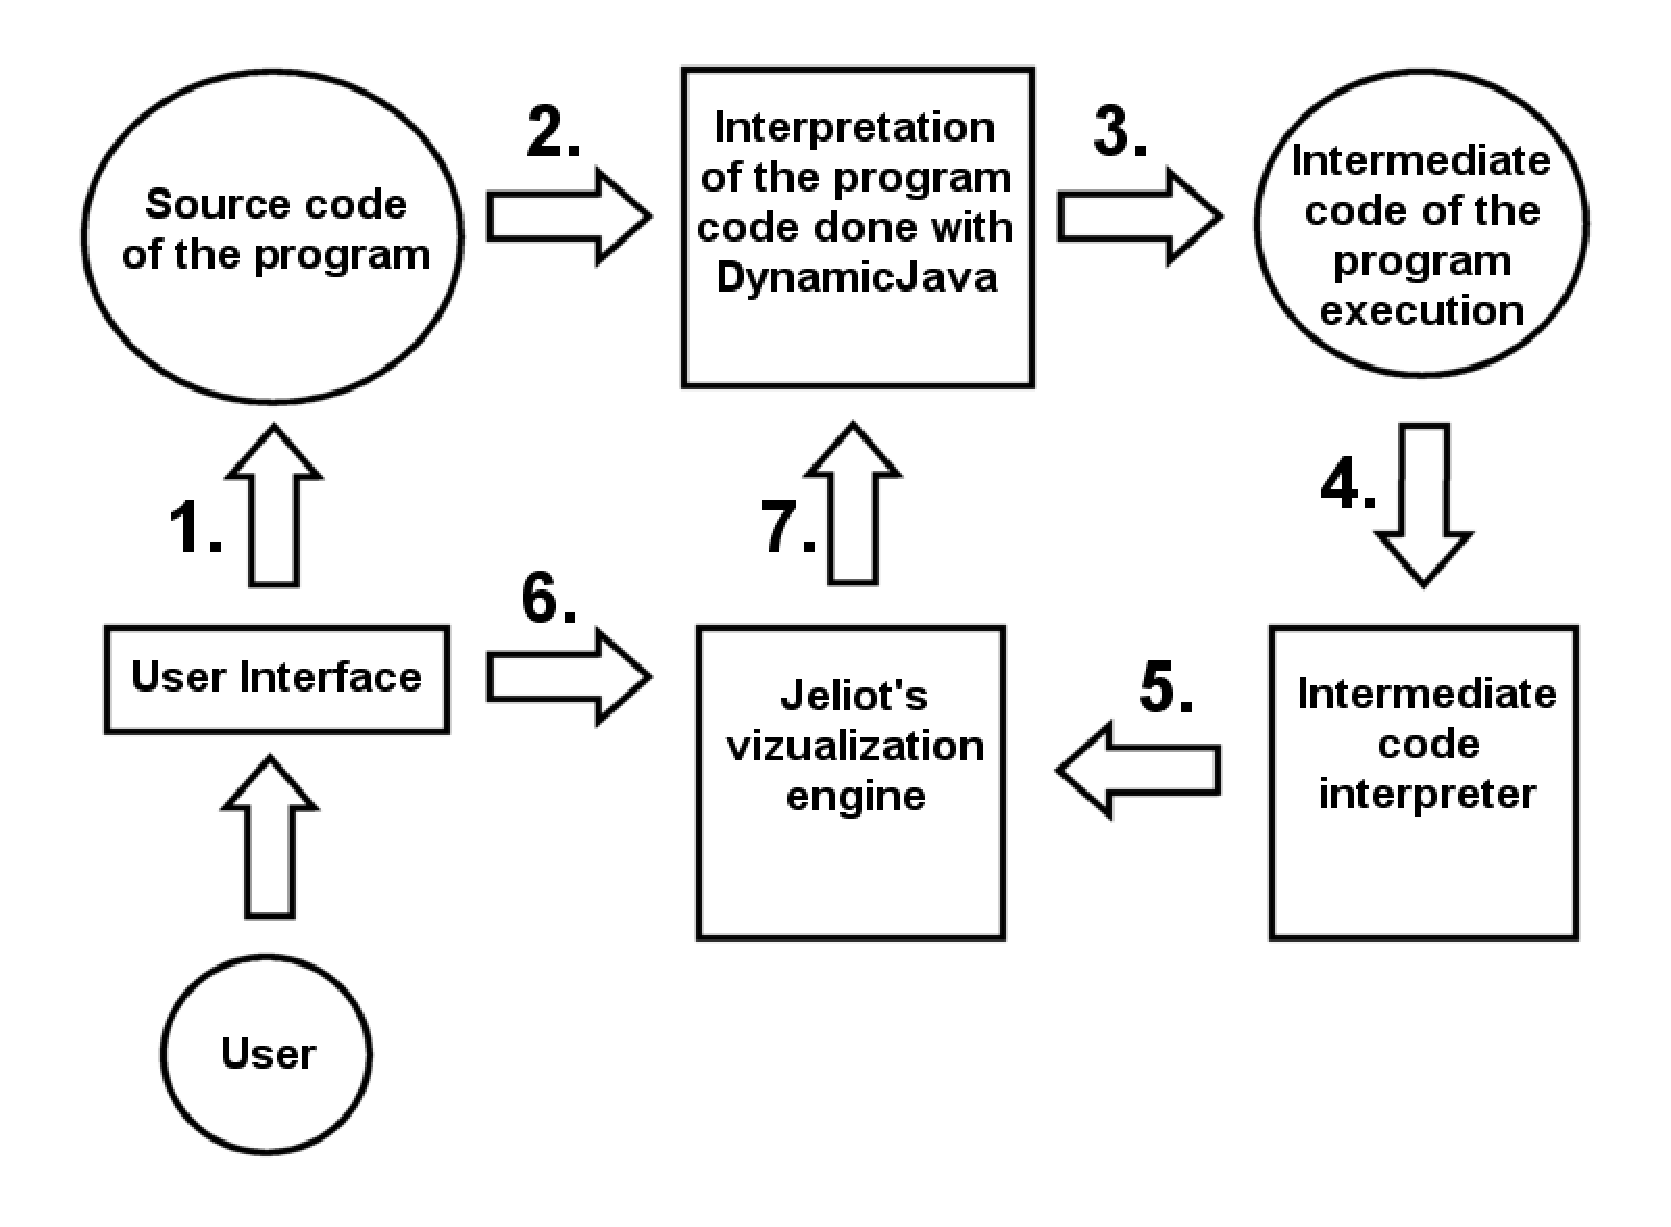
\includegraphics[height=10cm]{structure_of_jeliot_3.eps}
\caption{The functional structure of Jeliot~3.}
\label{fig:structure_of_jeliot_3}
\end{center}
\end{figure}

The functional structure of the Jeliot~3 is shown in the Figure~\ref{fig:structure_of_jeliot_3}.
A user interacts with the user interface and forms the source code of the program (1).
The source code is sent to the Java interpreter and the intermediate code is extracted (2 and 3).
The intermediate code is interpreted and the directions are given to the visualization engine (4 and 5).
A user can control the animation by playing, pausing, rewinding or playing step-by-step the animation (6).
Furthermore, the user can input data, for example, an integer or a string, to the program executed
by the interpreter (6 and 7).

